\documentclass[a4paper]{article}
\usepackage[T1]{fontenc}
\usepackage[utf8x]{inputenc}
\usepackage[english,russian]{babel}
\usepackage{multicol}
\usepackage{fancyhdr}
\usepackage[warn]{mathtext}
\usepackage{graphicx}
\usepackage{microtype}
\usepackage{wrapfig}
\usepackage{amsmath}
\usepackage{floatflt}
\usepackage{geometry} \geometry{verbose,a4paper,tmargin=2cm,bmargin=2cm,lmargin=1.5cm,rmargin=1.5cm}
\usepackage{float}
\usepackage{amssymb}
\usepackage{caption}
\usepackage{epsfig}
\usepackage{newunicodechar}
\usepackage{manfnt}
\usepackage{wasysym}

\begin{document}

\graphicspath{ {pictures/} }

\begin{titlepage}
	\centering
	\vspace{5cm}
    {\scshape\LARGE Московский физико-технический институт\par}
    

	\vspace{8cm}
	{\scshape\Large Лабораторная работа по вакуумной электронике \par}
	\vspace{2cm}
    {\huge\bfseries Растровый электронный микроскоп \par}
	\vspace{4cm}
	\vfill
\begin{flushright}
	{\large выполнил студент Б04-852 группы ФЭФМ}\par
	\vspace{0.3cm}
	{\LARGE Яромир Водзяновский}
\end{flushright}
	
	\vfill
Долгопрудный, 2020
% Bottom of the page
\end{titlepage}

\pagestyle{fancy} 
\fancyhead{}
\fancyhead[R]{Вакуумная электроника}
\fancyhead[L]{РЭМ $\sim  \hat(\, ^{\circ} 0  ^{\circ} \, \hat) \sim$}
% \fancyhead[LE,RO]{Квантовая физика   $ (^{/} \hat\; \omega  \hat\;) ^{/}$}
\fancyhead[C]{}
\fancyfoot[C]{ \noindent\rule{\textwidth}{0.4pt} \thepage }
% $\sim(\; ^{\circ }\omega   \; ) \sim$


\newpage

\section{Цель работы}

\begin{enumerate}
    \item Изучить физические принципы функционирования и основные методики измерений РЭМ
    \item Получить изображения различных образцов в следующих режимах работы РЭМ:
    \begin{itemize}
        \item режим сбора истинно вторичных электронов
        \item режим сбора упруго-отражённых электронов
    \end{itemize}
\end{enumerate}

\section{Физические основы растровой электронной микроскопии}
Принцип растровой электронной микроскопии состоит в сканировании исследуемой поверхности тонким электронным 
лучом по типу телевизионной развёртки. Выбитые электронным лучом вторичные электроны регистрируются детектором 
электронов. Интенсивность полученного с детектора сигнала определяет яркость точки растра на итоговом изображении. 
Так как коэффициент вторичной эмиссии зависит от угла падения первичных электронов, на экране монитора возникает 
изображение, определяемое рельефом исследуемой поверхности.

\subsection{Вторичная электронная эмиссия}

\textbf{Вторичная электронная эмиссия} - испускание электронов из твёрдого тела при бомбардировке пучком первичных электронов. 
Это явление представляет собой сложное наложение нескольких взаимосвязанных процессов: упругое и неупругое рассеяние первичных 
электронов, возбуждение внутренних, истинно вторичных электронов, их движения к поверхности и выхода в вакуум. Сложный характер 
явления вторичной электронной эмиссии проявляется в энергетическом спектре вторичных электронов (рис. \ref{spectr})

\begin{figure}[H]
    \centering
    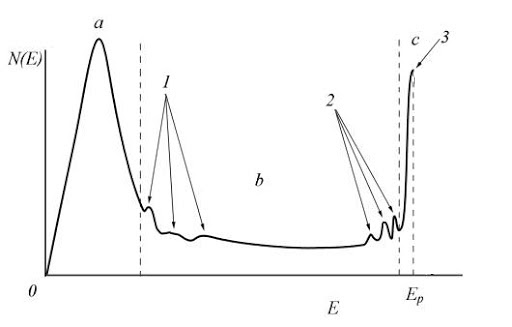
\includegraphics[scale = 2]{1.jpg}
    \caption{Качественный рисунок энергетического спектра вторичных электронов}
    \label{spectr}
    \end{figure}

\begin{itemize}
    \item первая область ($<50$ eV) - медленные истинно вторичные электроны).
    \item вторая область ($50 - 2000$ eV) - оже-электроны среди неупруго- и упруго-отражённых электронов 
    \item При энергии, близкой к энергии первичных электронов $E_0$, наблюдается узкий пик, соответствующий упруго отраженным электронам
\end{itemize}

Спектр \textbf{истинно вторичных электронов} имеет вид кривой с максимумом при некотором значении $E = E_m$. У металлов и полупроводников $E_m = 1.5 - 3$ эВ, 
полуширина спектра $\triangle E = 3 - 10$ эВ; у диэлектриков $E_m \approx 1$ эВ, полуширина спектра $\triangle E \approx 1.5 - 3$ эВ. Вторичная электронная 
эмиссия характеризуется коэффициентом вторичной эмиссии $\delta$, зависящим от элементного состава вещества и от угла падения пучка, то есть от рельефа поверхности. 
В частности, области на поверхности образца, на которые сканирующий пучок будет попадать под острыми углами, будут на изображении в РЭМ более светлыми. На рис. \ref{beta} 
изображена зависимость коэффициента вторичной эмиссии от энергии пучка. \par 

\begin{figure}[H]
    \centering
    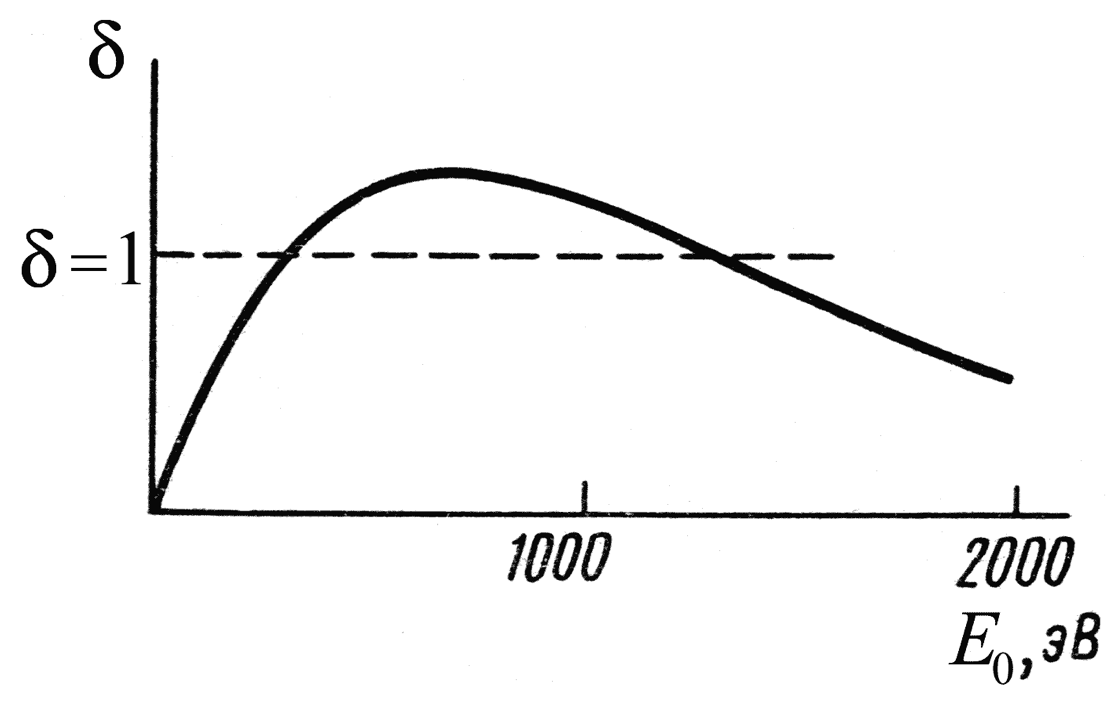
\includegraphics[scale = 0.2]{delta.png}
    \caption{Зависимость коэффициента вторичной эмиссии от энергии пучка.}
    \label{beta}
\end{figure}

Общий вид зависимости представлен на рис. выше. Вначале $\delta$ растёт вместе с E из-за увелечения числа вторичных электронов, затем с ростом глубины проникновения в вещество, 
$\delta$ начинает уменьшаться. Коэифцент вторичной эмисси зависит не только от вещества, но и от угла падения пучка $\delta (\varphi) = \frac{\delta(0)}{\cos \varphi}$, т.е.рельефа поверзности. Максимальный коэфицент будет в 
случае, если первичиный пучок пдаает на пучок практически параллельно поверхности.

В РЭМ также анализируются \textbf{отражённые электроны}. Коэффициент отражения - сложная функция $E_0$ и атомного номера $Z$ вещества. Если для малых энергий 
$E_0 = 0.6 - 3$ эВ для всех элементов максимум функции распределения соответствует упругоотражённым электронам, то для энергий $E_0 = 10 - 30$ кэВ максимум с ростом 
$Z$ растёт по величине и смещается в сторону $E_0$. При нормальном падении первичного пучка для всех элементов с ростом угла отражения уменьшается число отраженных 
электронов и сама величина максимума распределения.

\subsection{Контраст в растровом электронном микроскопе}

Информативными являются как отражённые, так и вторичные электроны. \par
Если образец однороден по составу и имеет выраженный рельеф, то изображение в \textbf{отражённых электронах} будет иметь такой же вид, как если бы мы смотрели на 
поверхность со стороны падения первичного пучка. Изображение также лишено полутонов и имеет чётко выраженные тёмные и светлые области. Для анализа образца, неоднородного 
по рельефу и составу, может использоваться парный детектор, на рис. \ref{signal1} изображен сигнал в зависимости от рельефа. \par

\begin{figure}[H]
    \centering
    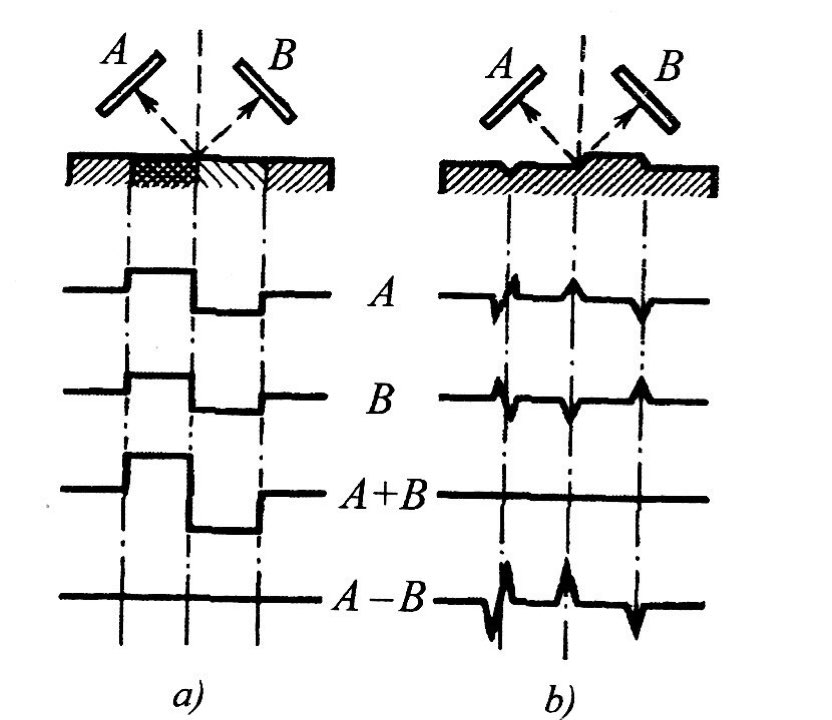
\includegraphics[scale = 0.2]{signal1_1.jpg}
    \caption{Принцип работы парного детектора при отраженных электронах}
    \label{signal1}
\end{figure}

В отличие от отражённых электронов, изображение в \textbf{истинно вторичных электронах} содержит полутона и имеет гораздо больше деталей, следовательно является более 
привычным для человеческого глаза. Большая глубина фокуса в РЭМ обусловлена тем, что между объектом и детектором вторичных электронов нет линзы с осесимметричным полем 
(в оптическом микроскопе линза между объектом и глазом присутствует). На рис. \ref{signal2} приведен пример изменения сигнала от рельефа.

\begin{figure}[H]
    \centering
    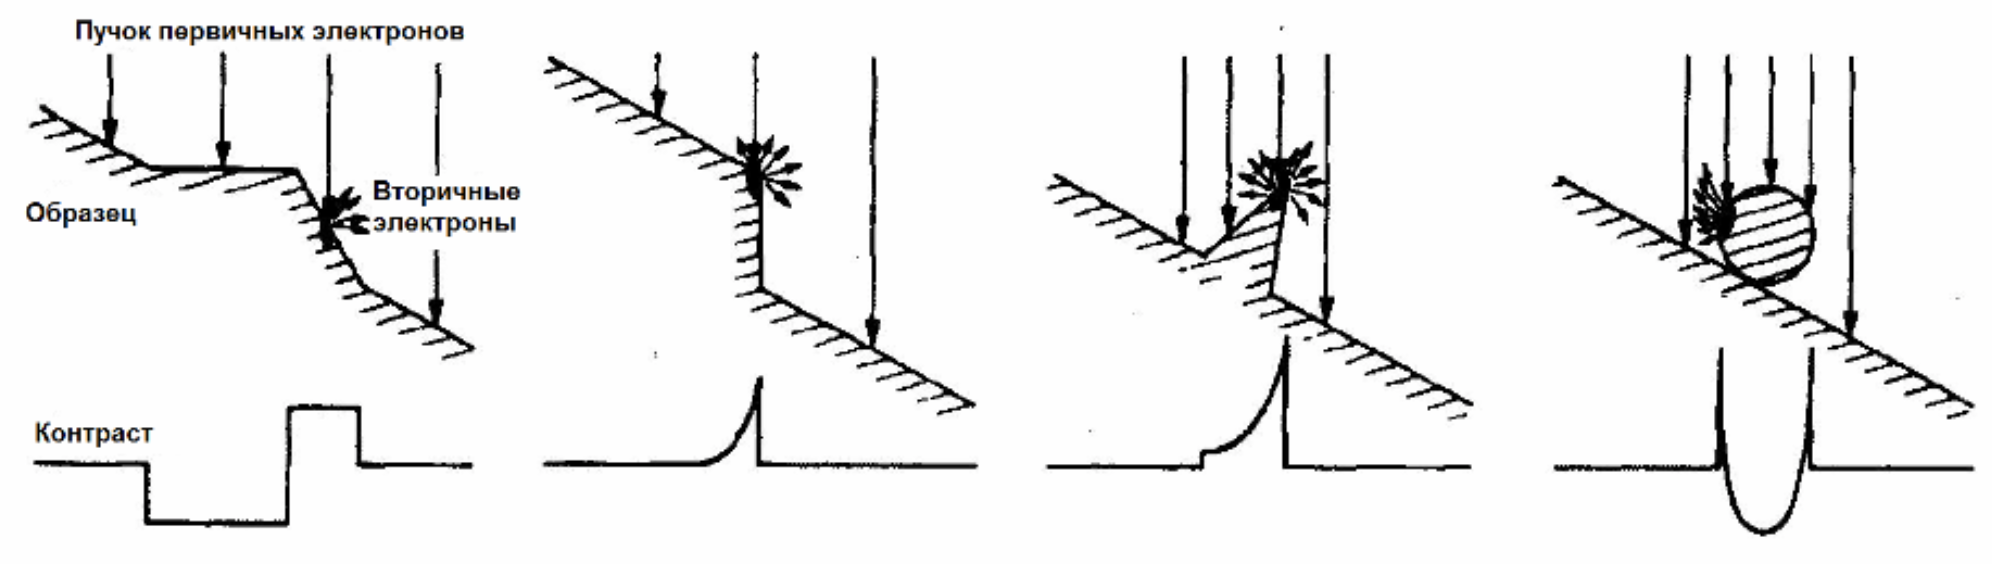
\includegraphics[scale = 0.5]{signal2.png}
    \caption{Изменение сигнала ВЭ из-за рельефа}
    \label{signal2}
\end{figure}

\subsection{Рентгеновский микроанализ}

Рентгеновский микроанализ в РЭМ осуществляется на основе следующих физических закономерностей и явления:

\begin{itemize}
    \item \textit{Закон Мозли} - зависимость энергии характеристического излучения от квадрата атомного числа элемента
    $$E  = R_1 (Z-\sigma)^2 \left ( \frac{1}{n_1^2} - \frac{1}{n_2^2} \right )$$
    \item \textit{Явление электронного удара} - электрон пучка с энергией несколько кэВ выбивает из атома К-электрон (или переводит его на один из высоких свободных уровней), 
    образуя вакансию. На образовавшуюся незанятую оболочку переходит один из L- или M-электронов, испуская рентгеновский фотон. На рис. \ref{series_1} изображена схема переходов.

    \begin{figure}[H]
        \centering
        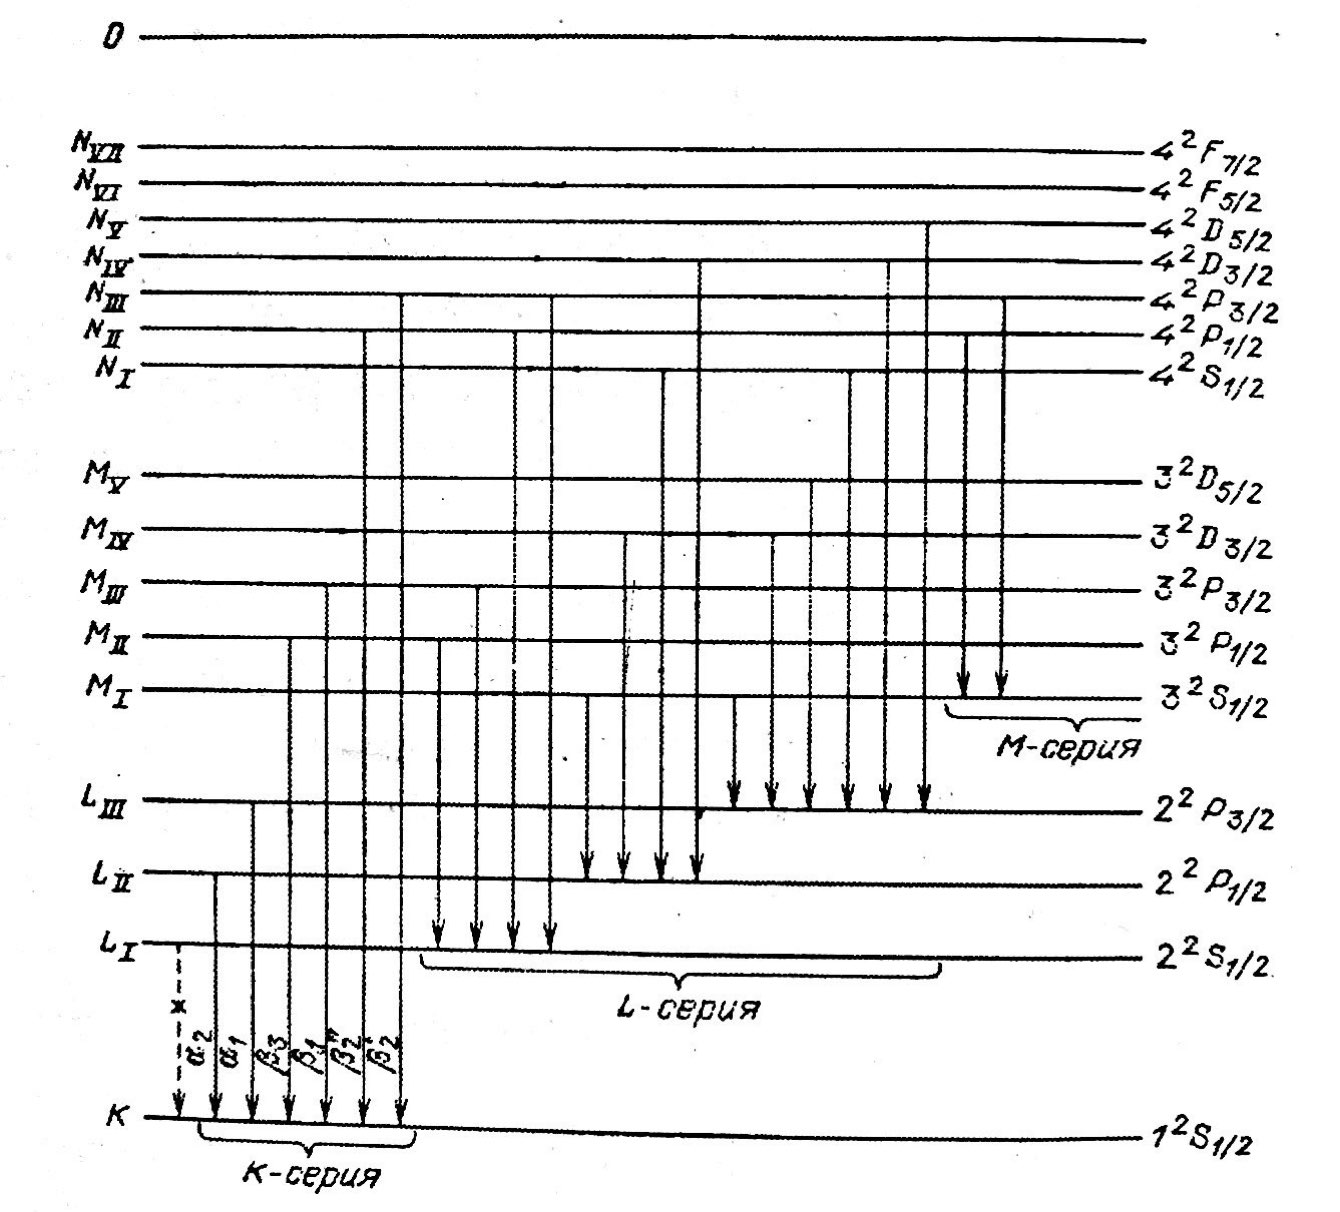
\includegraphics[scale = 0.2]{series_1.jpg}
        \caption{Схема переходов излучения характеристического рентгена.}
        \label{series_1}
    \end{figure}

    Эффективность такого возбуждения крайне низкая  - 1 к 1000 (число нужных фотонов к числу бомбардирующих электронов). Это происзодит по след. причинам:

    \begin{itemize}
        \item Электроны обыно взаимодействуют с поверхностными оболочками
        \item не усякая вакансия на К-оболочке приводит к жмисии рентген излучения.
        \item При взаимодействии жлектрона с ядром происзодит торможение первого и излучается непрерывный фон рентгеновского излучения - тормозного, который описывается приближенной формулой
        Крамерса:
        $$N(E) = \frac{a Z (E_0 - E)}{E}$$
        Она показывает число электронов в 1 сек. на единичный интервал энергий и на один падающий электрон с энергией $E_0$. 
        На рис. \ref{klines_1} показан этот спектр.

        \begin{figure}[H]
            \centering
            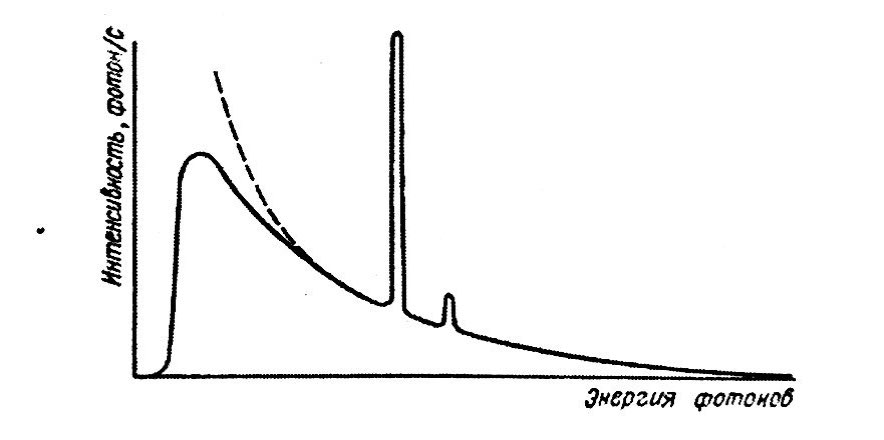
\includegraphics[scale = 0.2]{klines_1.jpg}
            \caption{Непрерывный спектр тормозного излучения и пик характеристической К-линии.}
            \label{klines_1}
        \end{figure}

    \end{itemize}

\end{itemize}

\section{Устройство и работа электронного растрового электронного микроскопа}

Структурная схема растрового электронного микроскопа представлена на рис. \ref{setup}. Ускорение и фокусировка пучка происходит в колонне, вверху которой находится электронная пушка, 
испускающая электроны. Далее следует система электронной оптики, которая формирует узки зонд, а также позволяет отклонять его в сторону, направляя в определенные точки образца. 
Во внутренних областях колонны поддерживается вакуум, чтобы избежать рассеяния электронов и окисления вольфрамовой нити, являющейся источником электронов. Образец, крепящийся 
в специальном держателе, окружен детектирующей аппаратурой - детектором отражённых электронов, детектором вторичных электронов, рентгеновским спектрометром.

\begin{figure}[H]
    \centering
    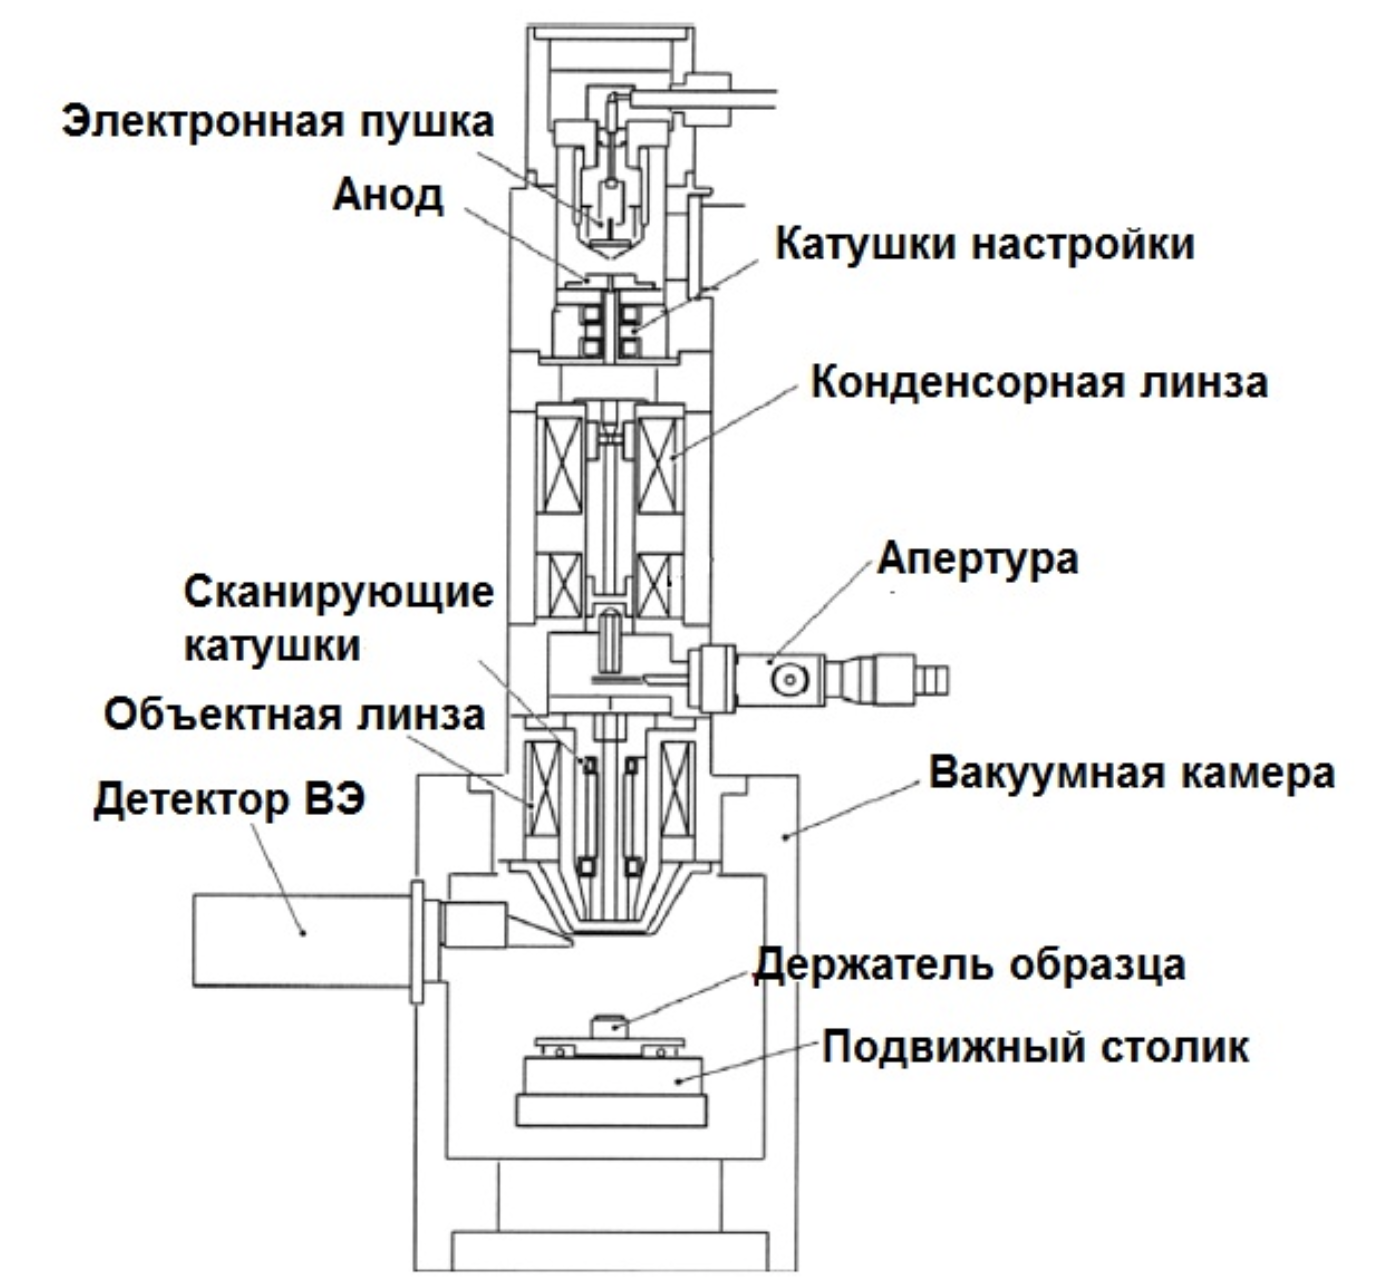
\includegraphics[scale = 0.3]{setup.png}
    \caption{Устройство РЭМ}
    \label{setup}
\end{figure}

\begin{itemize}
    \item эмиссия электронов в приборе осуществляется \textit{термоэлектронным катодом} из вольфрамовой проволоки
    \item далее электроны разгоняются до энергий до 30 кэВ с помощью системы из анода и катода
    \item пройдя через отверстие в анодной пластине, электроны попадают в \textit{систему электромагнитных линз}, с помощью которых формируется узкий зонд. Система 
    представляет собой цилиндрически симметричный электромагнит с очень острыми кольцевыми наконечниками полюсов, создающими сильное неоднородное магнитное поле, 
    фокусирующее электроны
    \item С помощью системы \textit{отклоняющих электромагнитных катушек} происходит сканирование пучка по поверхности образца
    \item \textit{детектор вторичных электронов} представляет собой сцинцилляторный счётчик. Вторичные электроны собираются у детектора с помощью клетки Фарадея. 
    Падающие на напылённый фосфором слой электроны вызывают испускание ультрафиолетовых фотонов, которые по световоду попадают в фотоумножитель
    \item для детектирования \textit{отражённых электронов} используется твердотельный детектор, который представляет собой кольцо, окружающее первичный пучек электронов.
    \item для проведения рентгеновского микроанализа образца используются \textit{волновые или дисперсионные детекторы} рентгеновского излучения

    \begin{itemize}
        \item \textbf{Волновой детектор} с помощью монохроматора (кристалл-детектор) выделяет из полного потока излучения лишь определенный длины волн из условия Брэгга-Вульфа, как известно,
        максимум для рентгеновского излучения будет достигаться при определенном угле:
        $$\lambda n = 2 d \sin \theta$$

        \item \textbf{Дисперсионный детектор} преобразует энергию каждого фотона в пропорциональный жнергии сигнал напряжения. Падающий рентген ионизирует атомы в кристалле-детекторе,
        в результате образуются неравновесные электроны и дырки. Затем с помощью предусилителя на полевом тразисторе неравновесный заряд преобразуется в сигнал напряжения. 
    \end{itemize}

    \item Для выбора времени сканирования пользуются соотношением сигнал шум:
    $$S/N = \frac{n}{\sqrt(n)} = \sqrt(n)$$
    Из полученной оценки на число электронов, падающих на поверхность и значения тока зонда находят время сканирования одной точки. n - число первичных электронов. 

\end{itemize}

\section{Ход работы}

\begin{enumerate}
    \item Получим изображение таблетки смеси двух металлов - меди и хрома в режиме детектирование истинно вторичных электронов. рис. \ref{tablet01}.
    
    \begin{figure}[H]
        \centering
        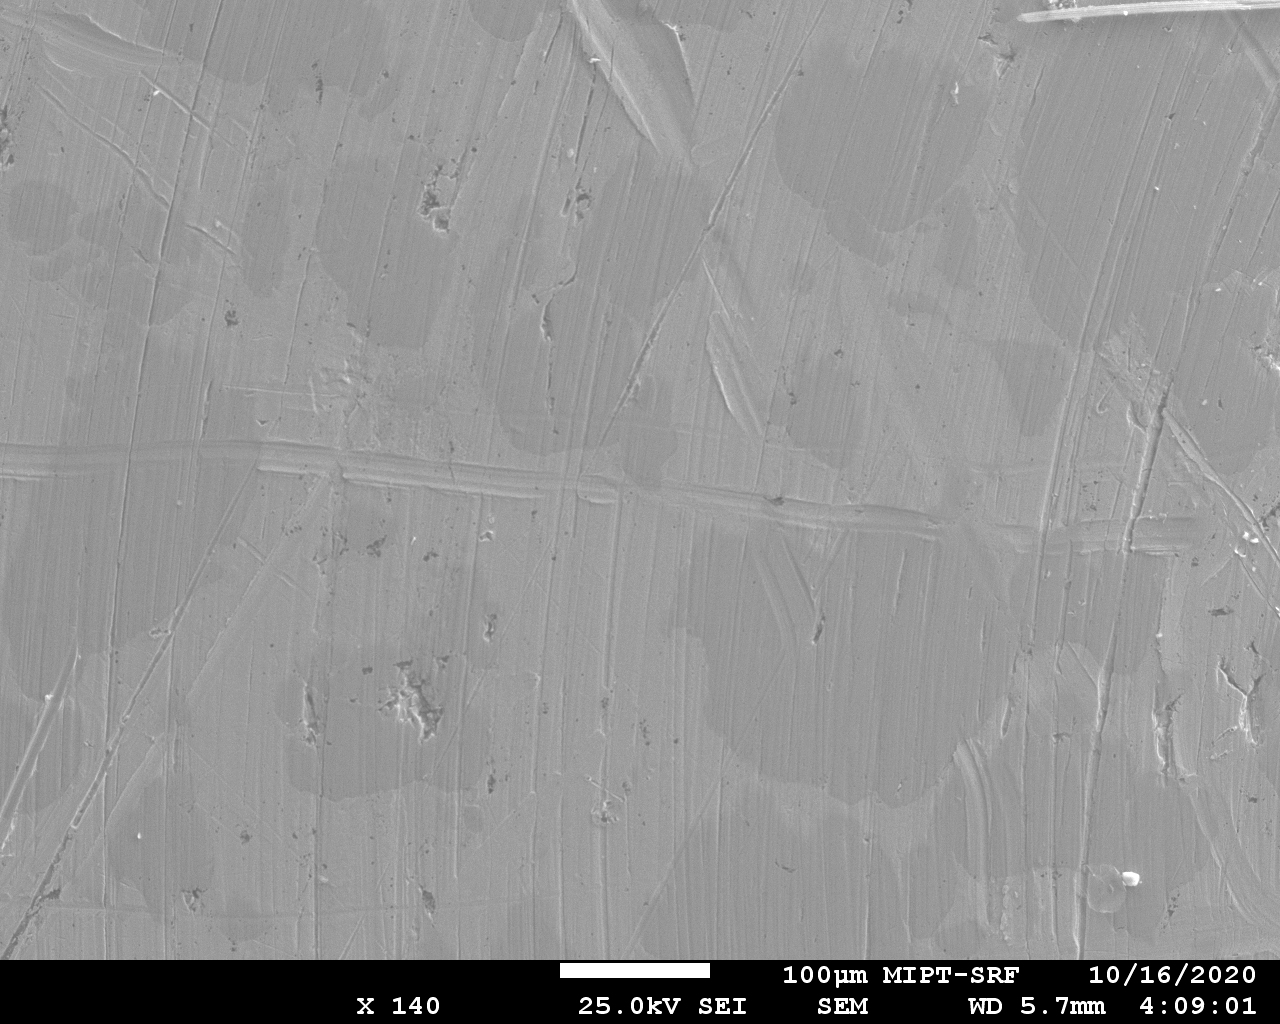
\includegraphics[scale = 0.9]{Tablet01.jpg}
        \caption{Таблетка медь/хром}
        \label{tablet01}
    \end{figure}

    Мы наблюдаем как микрорельеф, так и контраст обусловленный разным составом таблетки, это возможно, т.к есть зависимость коэффициента истинно вторичных электронов от атомного номера.

    \item В режиме сбора истинно вторичных электронорв получим изображения крла бабочки с разным временем сканирования и разным увеличением.
    
    \begin{figure}[h]
        \begin{center}
        \begin{minipage}[h]{0.45\linewidth}
        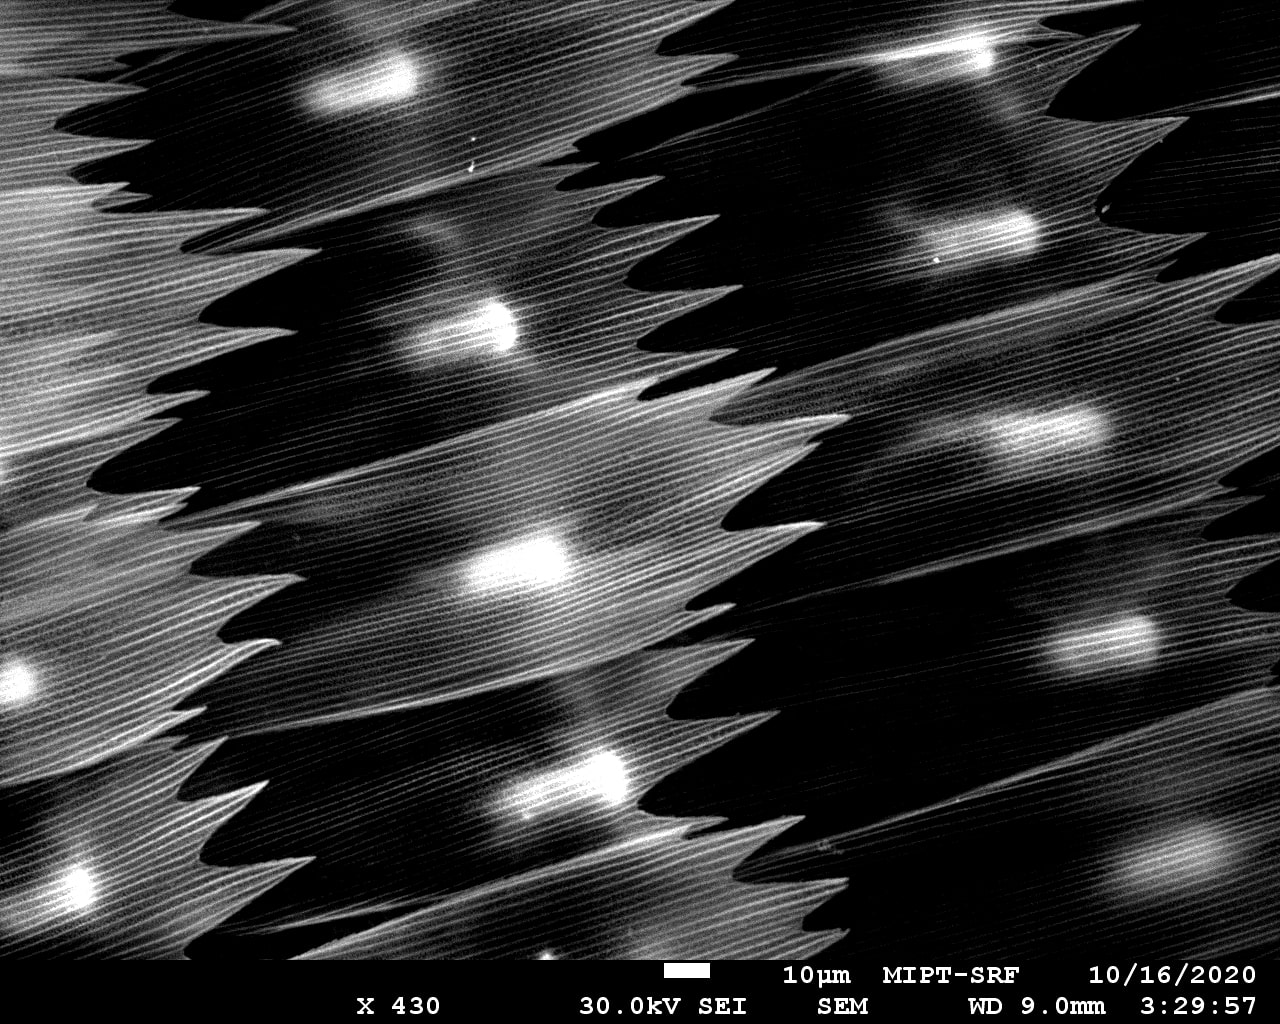
\includegraphics[width=1\linewidth]{Buterfly01.jpg}
        \caption{} 
        \label{Buterfly01}
        \end{minipage}
        \hfill 
        \begin{minipage}[h]{0.45\linewidth}
        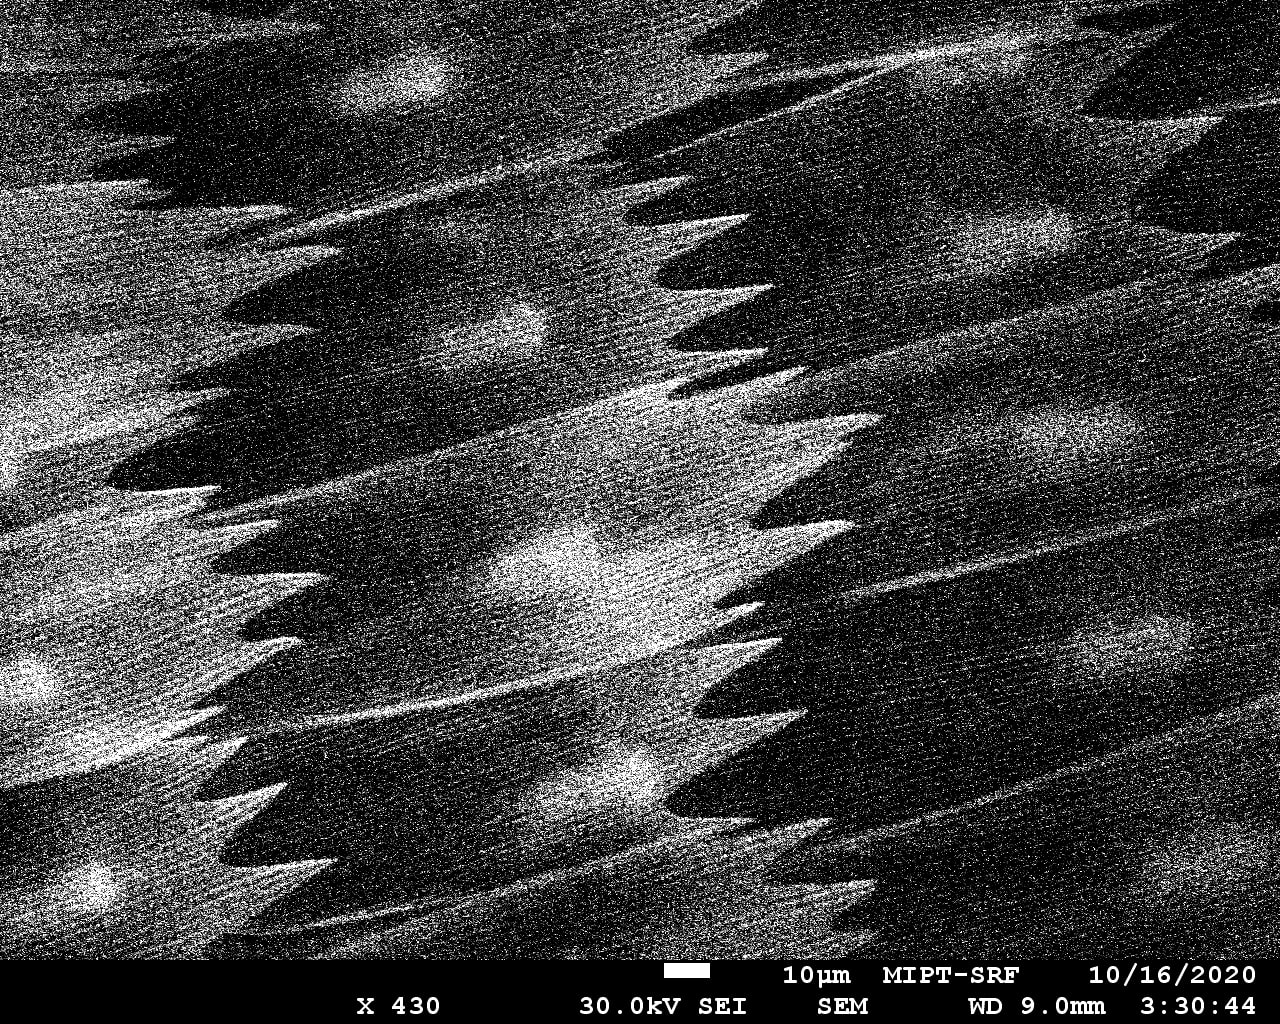
\includegraphics[width=1\linewidth]{Buterfly02.jpg}
        \caption{}
        \label{Buterfly02}
        \end{minipage}
        \end{center}
    \end{figure}

    \begin{figure}[H]
        \begin{center}
        \begin{minipage}[h]{0.45\linewidth}
        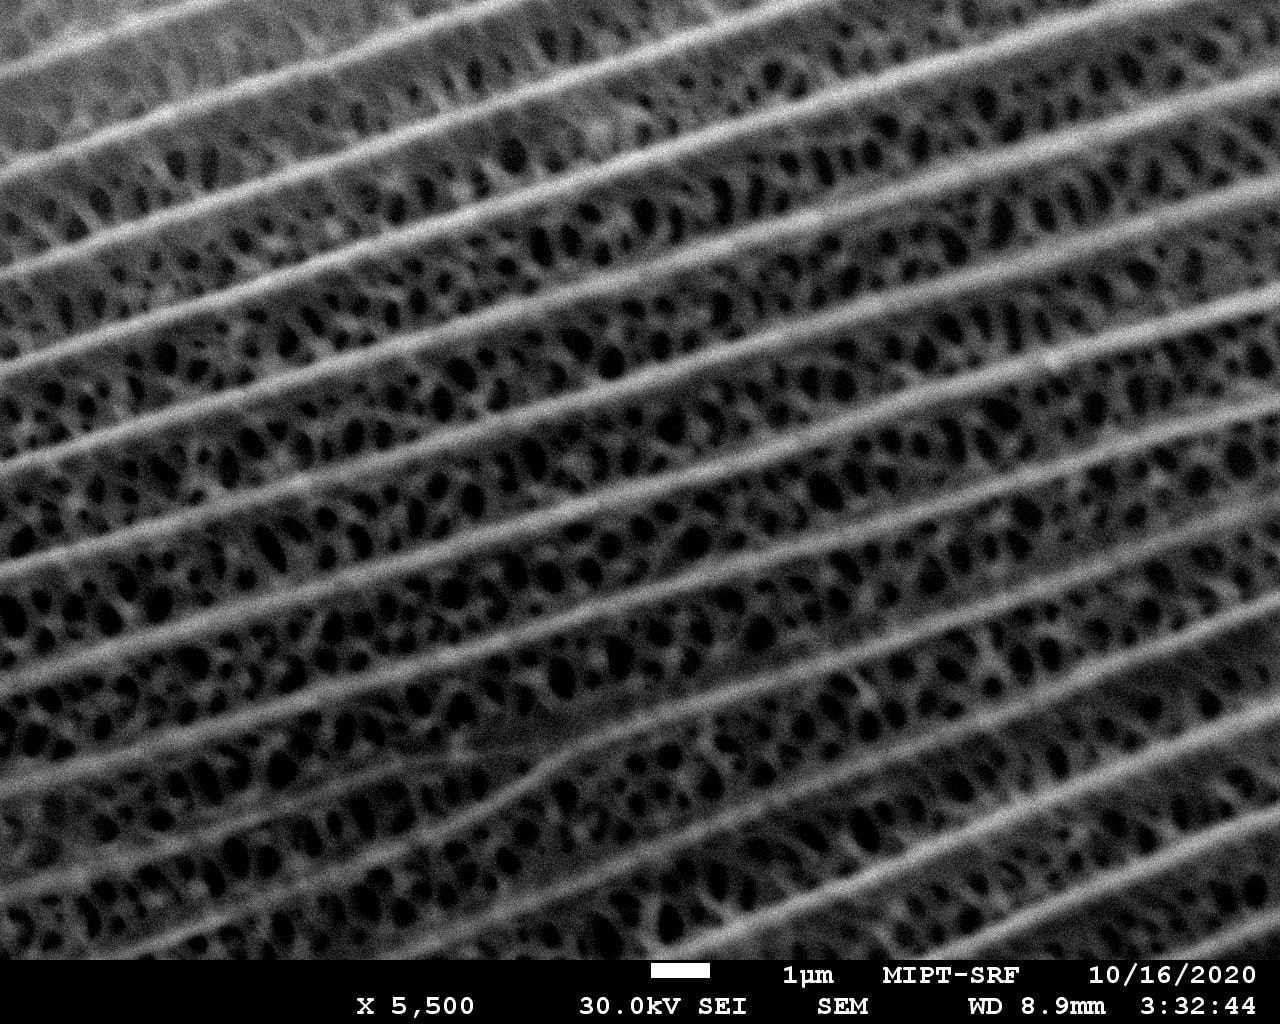
\includegraphics[width=1\linewidth]{Buterfly03.jpg}
        \caption{} 
        \label{Buterfly03}
        \end{minipage}
        \hfill 
        \begin{minipage}[h]{0.45\linewidth}
        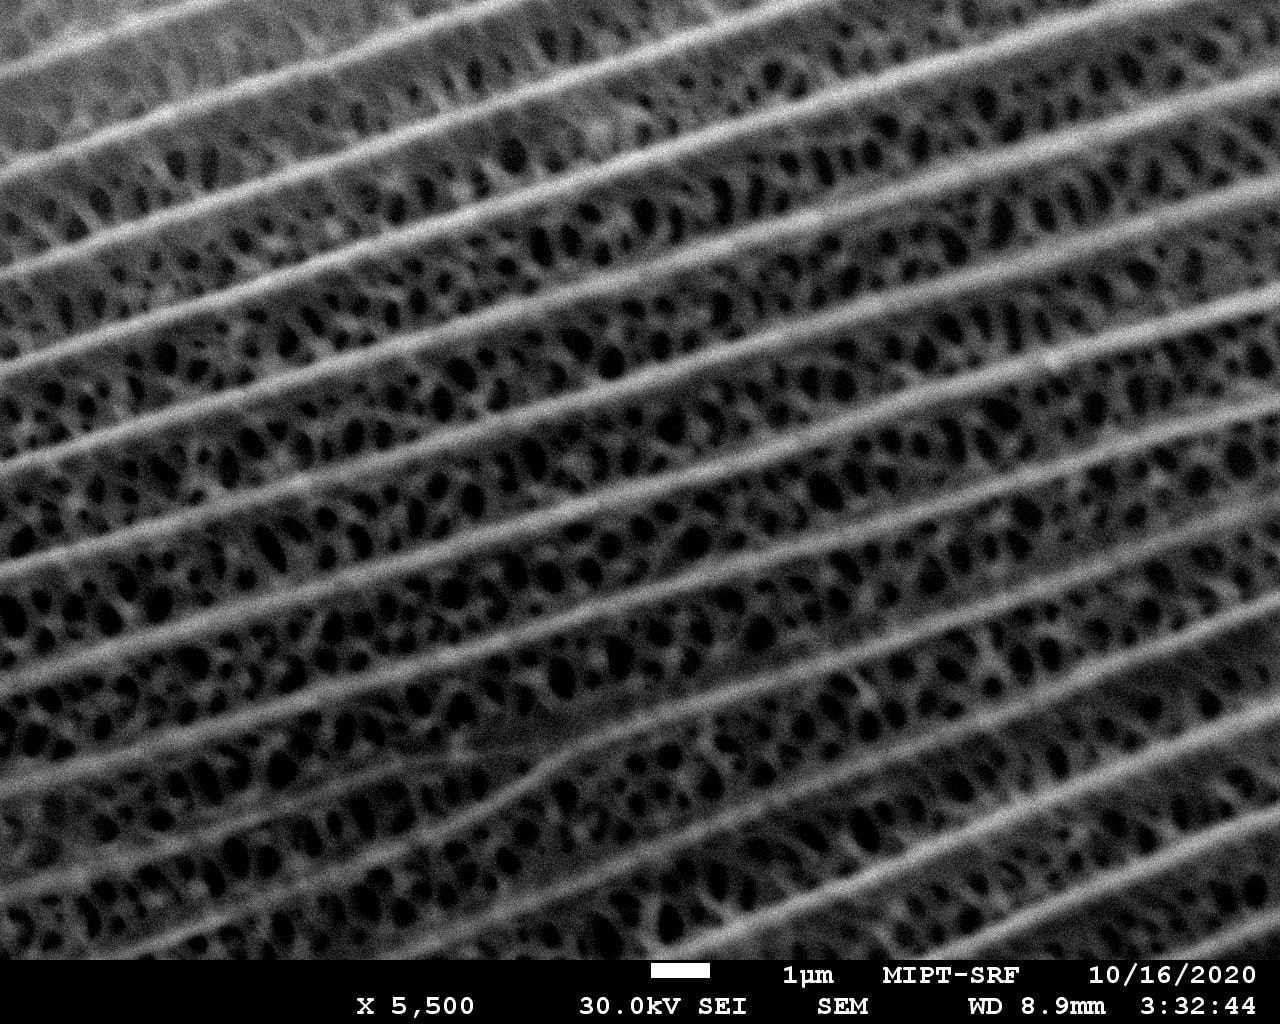
\includegraphics[width=1\linewidth]{Buterfly03.jpg}
        \caption{}
        \label{Buterfly04}
        \end{minipage}
        \end{center}
    \end{figure}
    
    \begin{figure}[H]
        \centering
        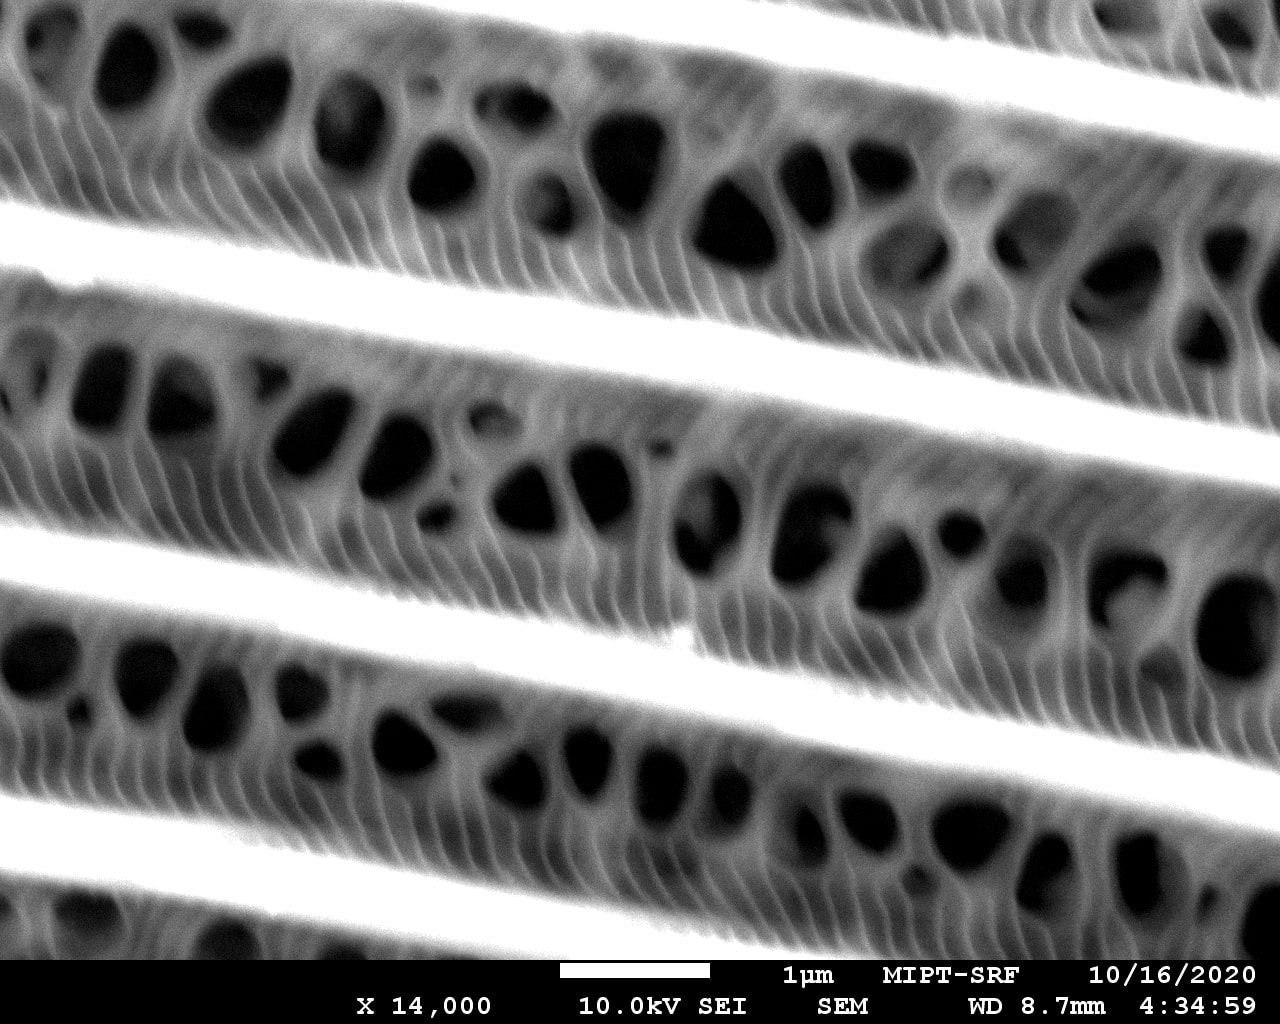
\includegraphics[scale = 0.2]{Buterfly05.jpg}
        \caption{}
        \label{Buterfly05}
    \end{figure}


    \item Получим изображение кусочка пенопласта, который является диэлектриком, соответственно при бомбардировке электронами, он начнет заряжаться 
    (момент во время зарядки на рис. \ref{foam}), после того как он достаточно зарядится, почти все бомбардирующие жлкетроны будут отражатся от пеноплатса и стенок камеры и попадать на детекторы,
    и мы увидим изображение камеры со стороны образцов рис. \ref{foam01}

    \begin{figure}[H]
        \begin{center}
        \begin{minipage}[h]{0.45\linewidth}
        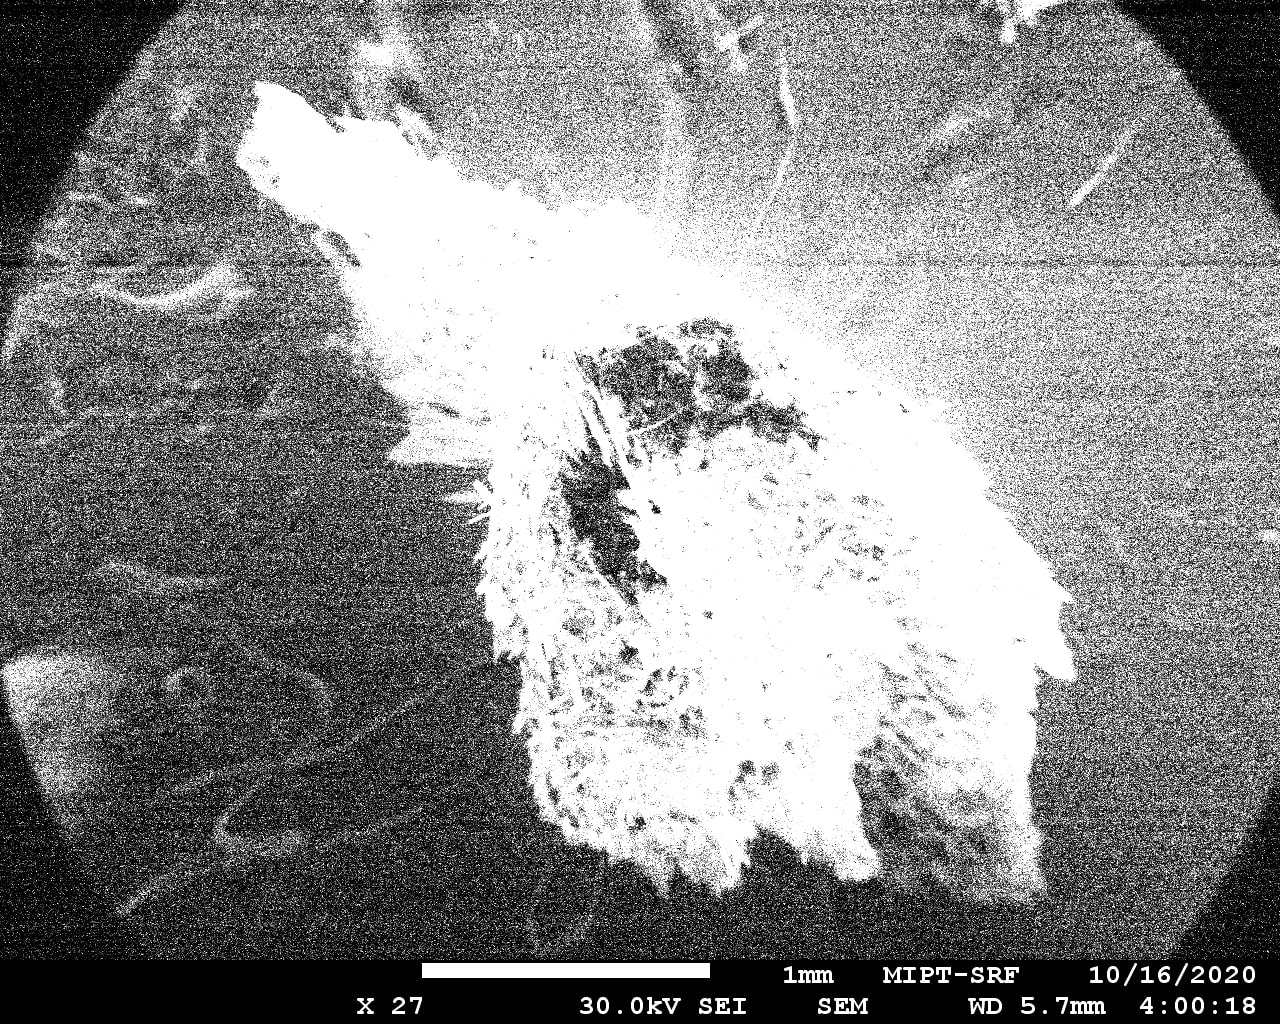
\includegraphics[width=1\linewidth]{Foam.jpg}
        \caption{} 
        \label{foam}
        \end{minipage}
        \hfill 
        \begin{minipage}[h]{0.45\linewidth}
        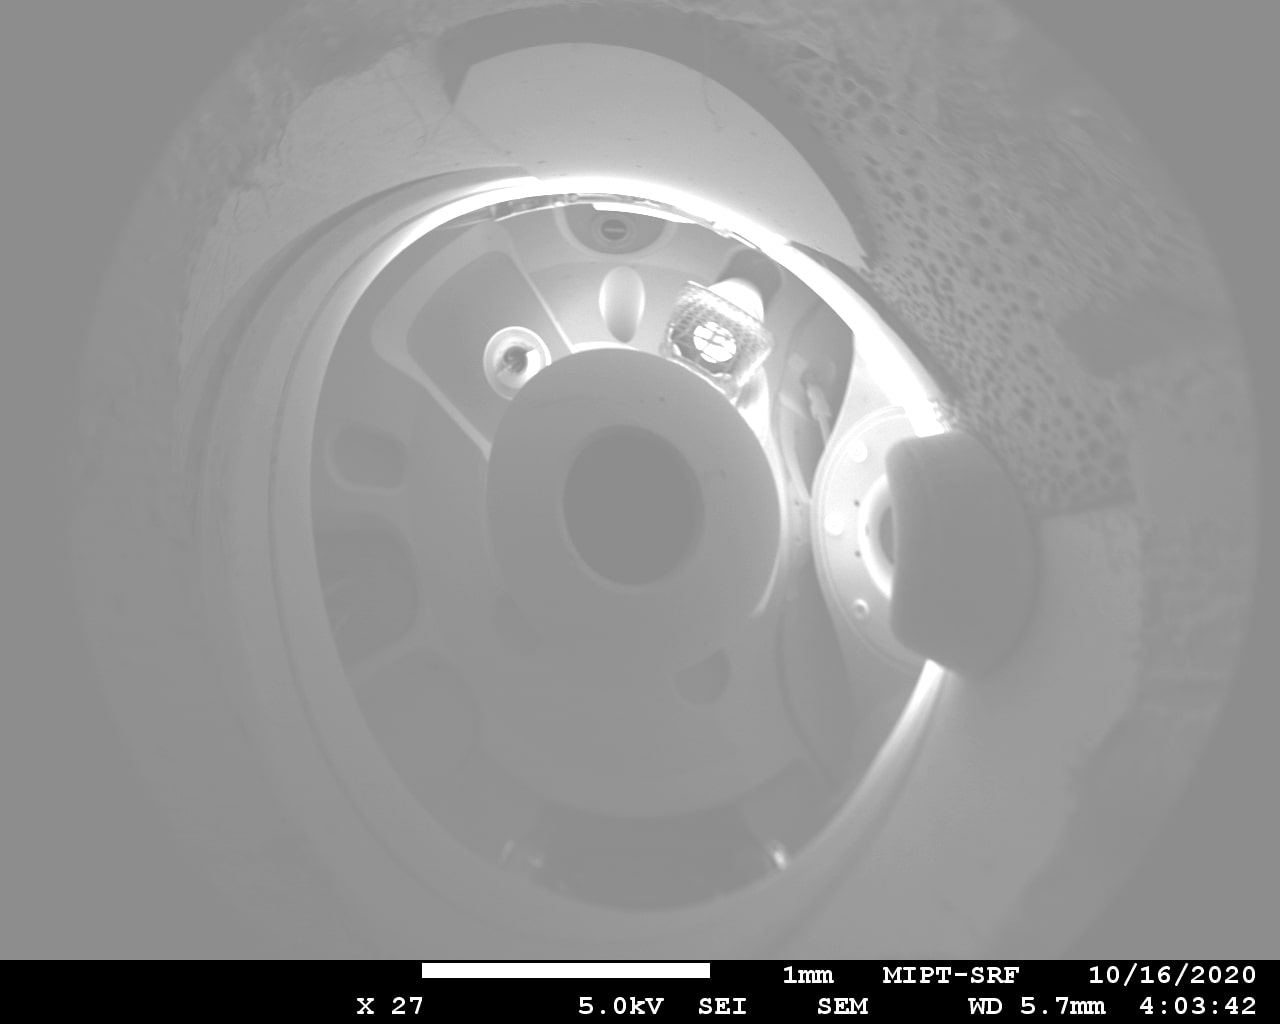
\includegraphics[width=1\linewidth]{Foam01.jpg}
        \caption{}
        \label{foam01}
        \end{minipage}
        \end{center}
    \end{figure}



    \item В режиме сбора обратно рассеяных электронов получим изображение кристаллической решетки $SiO_2$ на рис. \ref{sio1} и рис. \ref{sio2}. 
    
    \begin{figure}[H]
        \begin{center}
        \begin{minipage}[h]{0.45\linewidth}
        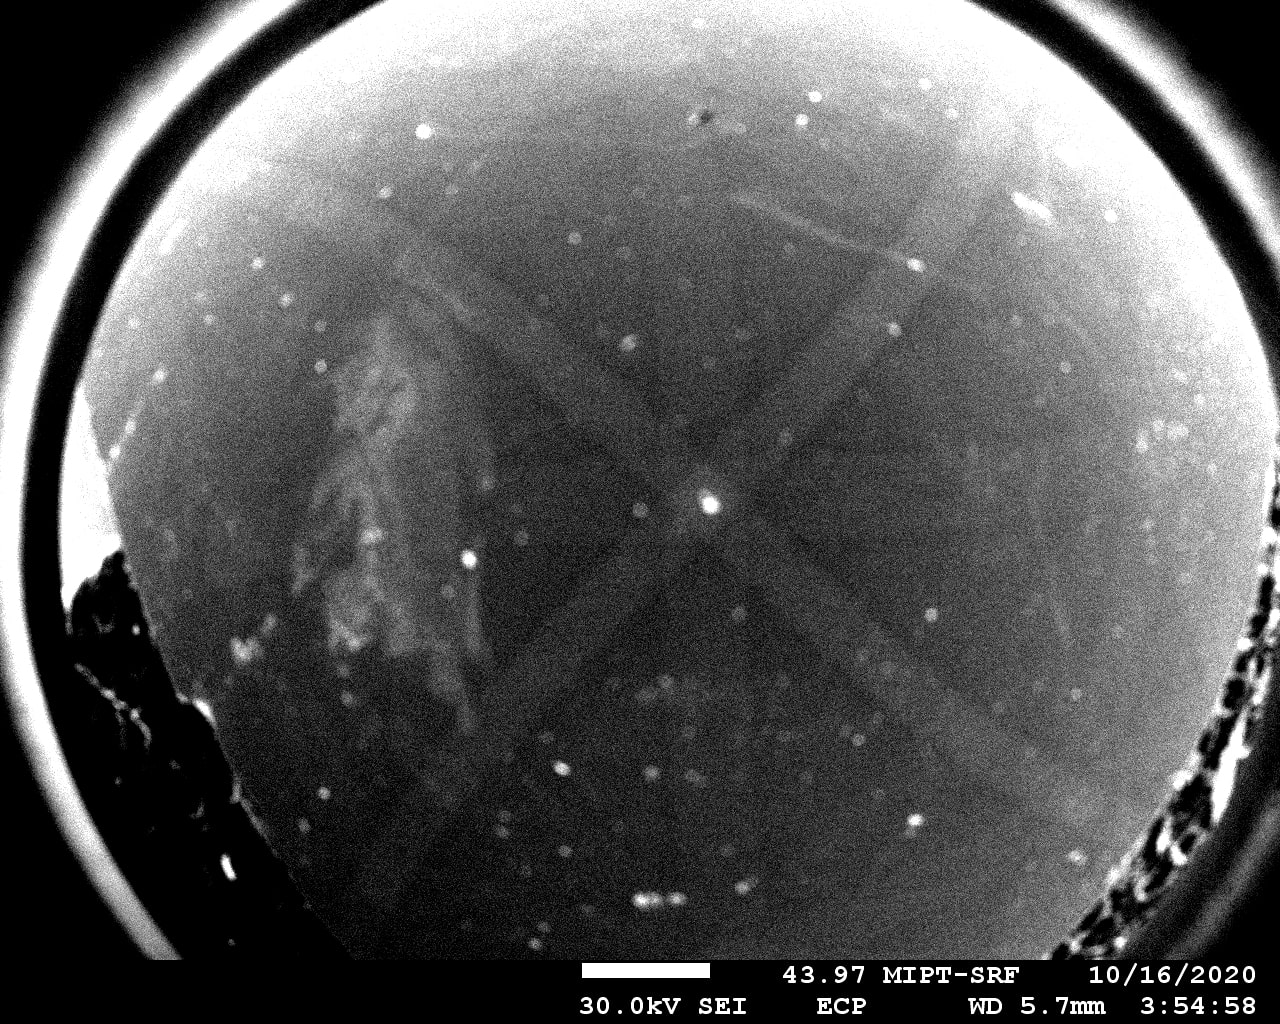
\includegraphics[width=1\linewidth]{Si01.jpg}
        \caption{} 
        \label{sio1}
        \end{minipage}
        \hfill 
        \begin{minipage}[h]{0.45\linewidth}
        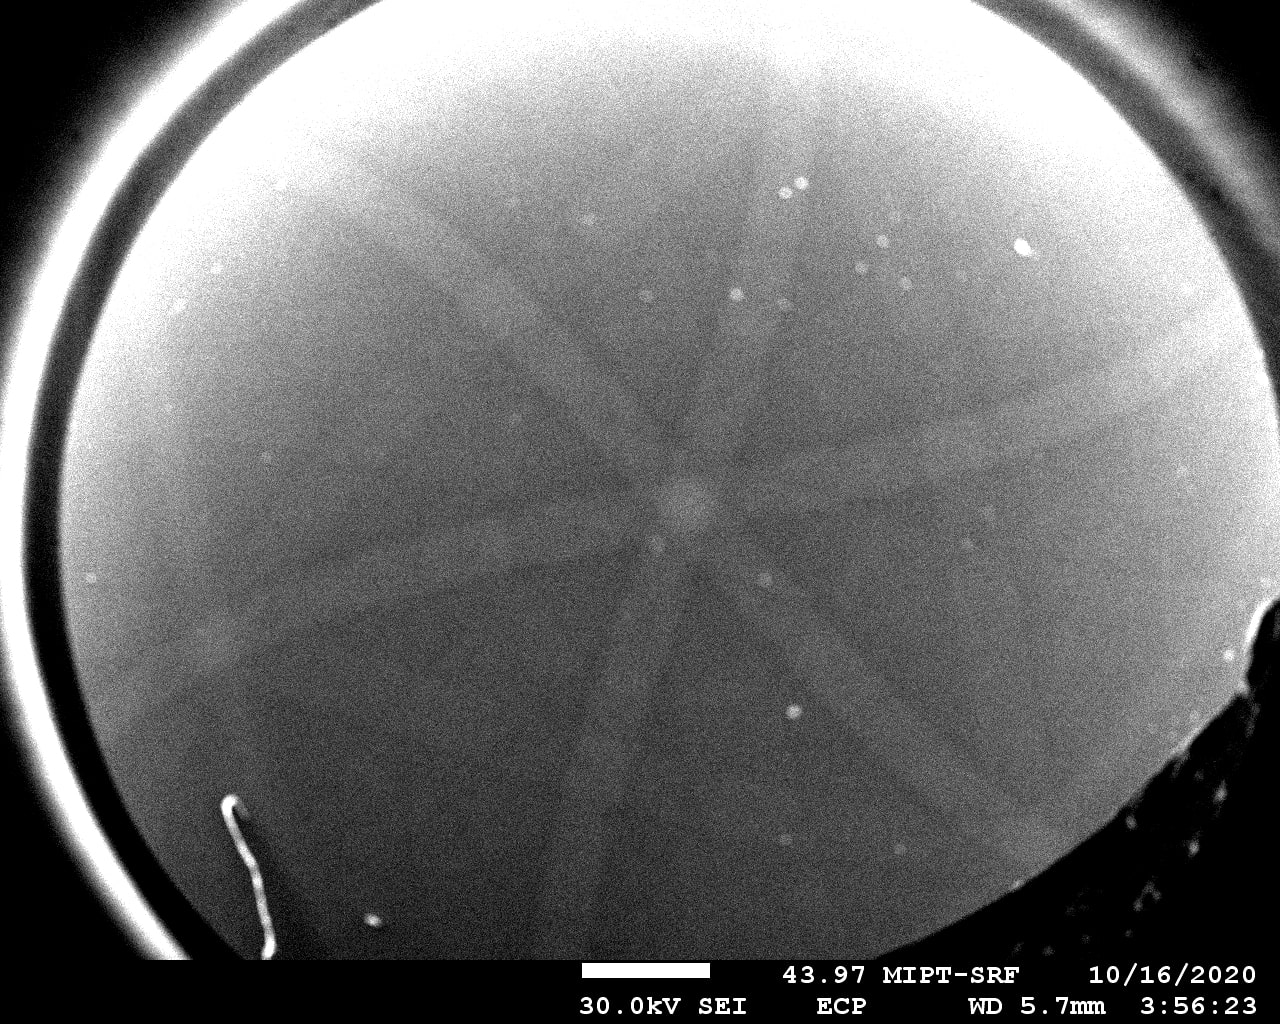
\includegraphics[width=1\linewidth]{Si02.jpg}
        \caption{}
        \label{sio2}
        \end{minipage}
        \end{center}
    \end{figure}

    Это аномальная способность изменять коэффициент отражения при определенных орейнтациях монокристалла относительно первичного пучка. 
    Это связано с эффектом каналирования первичных электронов. То есть электроны движуться по каналам , образованными параллельными друг другу рядами атомов.

\end{enumerate}

\section{Вывод}

В ходе работы были изучены физические принципы работы растрового электронного микроскопа, а также его устройство. Были исследованы образцы сплава медь-хром, 
кусочек пенопласта, получено изображение кристаллической решетки монокристалла $SiO_2$, а также крыло бабочки в режиме сбора истинно вторичных электронов, а также в режиме сбора обратно рассеяных электронов.

\end{document}